\section{Evaluation}

We evaluate our counterfactual query rewriting approaches in the LongEval scenario that comes with overlapping queries across 6~timestamps between June~2022 and August~2023~\cite{alkhalifa:2023,alkhalifa:2024,galuscakova:2023}. First, we modify the LongEval datasets to focus on queries that re-occur across timestamps and subsequently study how documents evolve over time due to creations, deletions, and content updates. Finally, we evaluate the retrieval effectiveness of all approaches and use an ablation study to study if they generalize beyond previously known relevant documents.

\subsection{Experimental Setup}

% We modify the LongEval corpora~\cite{alkhalifa:2023,alkhalifa:2024,galuscakova:2023} to evaluate retrieval effectiveness for re-occuring queries over time. 
LongEval provides queries, documents, and relevance judgments derived with click models for June~2022, July~2022, September~2022, January~2023, June~2023, and August~2023. The queries and clicks were sampled from Qwant so that the queries rather do not change their intent over time~\cite{galuscakova:2023} while documents might be updated, deleted, or newly created. For each timestamp, we remove queries that did not occur in an earlier timestamp, leaving us with 5~timestamps for evaluation between July~2022 and August~2023~(between 169~and 298~test queries; June~2022 is skipped as no previous logs are available). Figure~\ref{fig:query-overlap} provides an overview of the re-occuring queries between the different timestamps. For instance, 138~queries from June~2023 re-occur in August~2024, forming the biggest time gap in our evaluation scenario, whereas the smallest time gap occurs for the 150~queries from June~2023 that re-occur in July~2023.

In our retrieval experiments, we contrast five baselines with our three approaches. We use BM25~\cite{robertson:1994}, BM25 with RM3 expansion (both implemented in PyTerrier~\cite{macdonald:2020}), ColBERT~\cite{khattab:2020}, List-in-T5~\cite{tamber:2023}, and monoT5~\cite{nogueira:2020}. We leave all baselines at their default hyperparameters. We also implement our three approaches in PyTerrier using BM25 as the underlying retrieval model. For boosting (BM25$_{Boost}$), we set $\lambda=0.7$ and $\mu=2$ based on previous experiments~\cite{keller:2024b}. For relevance feedback (BM25$_{RF}$), we use $k=10$ feedback terms as this is the default for RM3 in PyTerrier. For keyqueries (BM25$_{keyquery}$), we use {\color{red} TODO: Hyperparameter}.

%TODO: for camera ready: ColBERT, List-in-T5, and monoT5 baselines come from TIRA/TIREx


\begin{figure}[t]
    \begin{minipage}{.49\textwidth}
        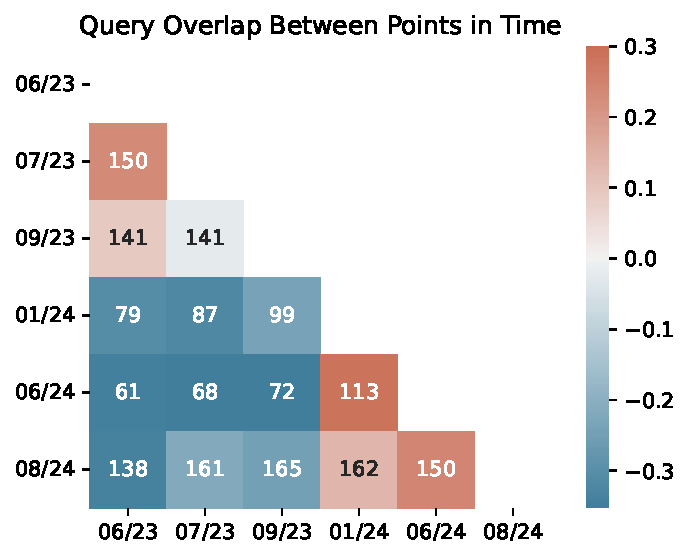
\includegraphics[width=\textwidth]{query-overlap}
        \vspace{-4ex}
        \caption{Frequency of queries over time.}
        \label{fig:query-overlap}
    \end{minipage}
    \hfill    
    \begin{minipage}{.49\textwidth}
        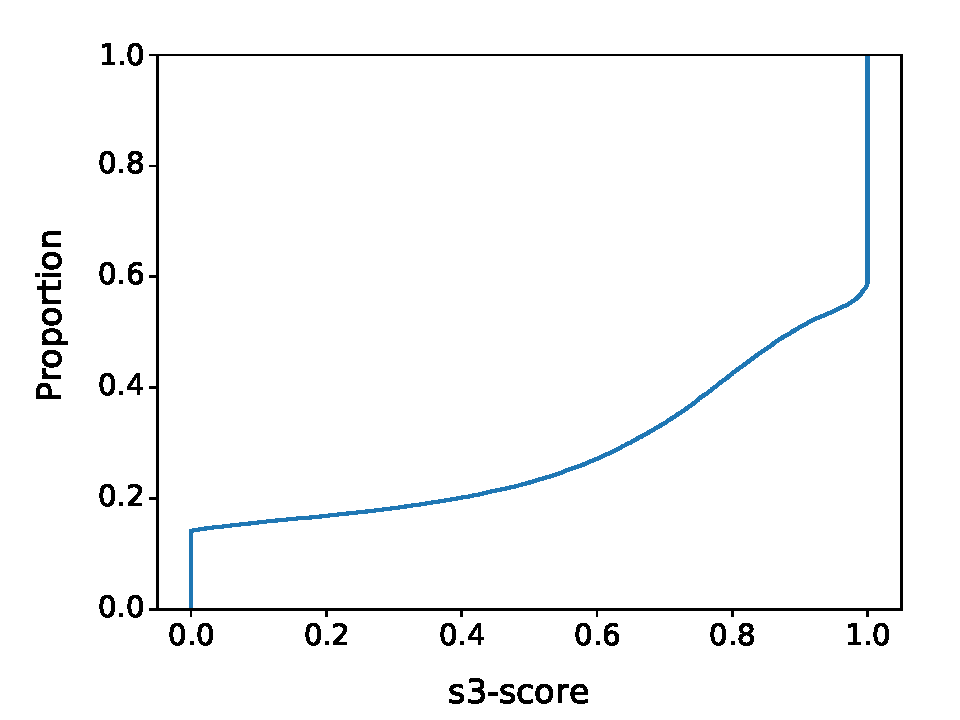
\includegraphics[width=\textwidth]{document-similarities}
        \vspace{-4ex}
        \caption{S$_{3}$ Similarities of documents with overlapping URLs as eCDF plot.}
        \label{fig:document-similarities}
    \end{minipage}
\end{figure}

\subsection{Evolution of Documents in the LongEval Corpora over Time}

After we fixed the queries to those that overlap among the different timestamps, only documents and qrels may evolve over time. Documents may evolve via deletion, creation, or updates to the content. Over time, between one and 2.5~million documents were available. Across all timestamps, 1.7~million documents were deleted over time, 2.6~million documents were newly created at some timestamp. For documents that occur across multiple timestamps, we measure how they changed over time by inspecting their pairwise similarities. We use the $S_{3}$ score~\cite{bernstein:2005} implemented in CopyCat~\cite{froebe:2021a} in default configuration to measure similarity (1~indicates identical documents, 0~documents without any overlap) as this score was specifically developed to identify redundant documents within retrieval scenarios~\cite{bernstein:2005}. Figure~\ref{fig:document-similarities} shows the $S_{3}$ similarities for all documents with overlapping URLs across all timestamps, indicating that 40\,\% of documents do not change their content~($S_{3}=1.0$), whereas around 50\,\%have an $S_{3}$ similarity below~0.8 that indicate non-negligible changes (prior research used 0.82~as near-duplicate threshold on Web corpora~\cite{froebe:2021a}). Given that the LongEval corpora evolve only slightly among the timestamps, we include an ablation study that removes all overlap to analyze how approaches generalize.



\subsection{Retrieval Effectiveness}


\begin{table}[t]
\small
\centering
\renewcommand{\tabcolsep}{3.2pt}
\caption{Retrieval effectiveness of the five baselines and our three approaches measured as nDCG@10 with and without unjudged documents (nDCG@10$^{'}$) across the five LongEval timestamps. {\color{red} $^{*}$ marks Bonferroni corrected significance for students t-test.}}
\label{tab:table-results}

\begin{tabular}{@{}l@{}cccccccccc@{}}
    \toprule
    \bfseries System & \multicolumn{5}{c}{\bfseries nDCG@10} & \multicolumn{5}{c}{\bfseries nDCG@10$^{'}$}\\
    \cmidrule(r@{.25em}){2-6}
    \cmidrule(l@{.25em}){7-11}
    
    & 07/22 & 09/22 & 01/23 & 06/23 & 08/23 & 07/22 & 09/22 & 01/23 & 06/23 & 08/23\\
    
    \midrule

    BM25 & .155 & .184 & .172 & .175 & .134 & .471 & .492 & .516 & .486 & .379 \\
    BM25$_{RM3}$ & .147 & .181 & .163 & .174 & .134 & .478 & .490 & .524 & .492 & .388 \\
    ColBERT & .198 & .207 & .201 & .184 & .151 & .402 & .409 & .420 & .408 & .315 \\
    List-in-T5 & .203 & .204 & .202 & .198 & .161 & .401 & .413 & .425 & .413 & .317 \\
    monoT5 & .202 & .219 & .197 & .202 & .154 & .405 & .410 & .415 & .411 & .314 \\
    
    \midrule
    
    BM25$_{Boost}$ & .355 & .372 & .287 & .364 & .271 & .529 & .546 & .541 & .540 & .412 \\
    BM25$_{RF}$ & .303 & .332 & .241 & .262 & .191 & .606 & .611 & .590 & .552 & .426 \\
    BM25$_{keyquery}$ & .252 & .285 & .219 & .224 & .162 & .533 & .549 & .552 & .523 & .406 \\

\bottomrule
\end{tabular}
\end{table}


We evaluate the effectiveness of our five baselines and our three approaches using nDCG@10. However, as the LongEval corpus was derived from click logs derived from unknown rankings, unjudged documents have a high impact on the evaluation. In this scenario, it is recommendet to remove unjudged documents to mitigate their impact~\cite{sakai:2007} which we additionally report as nDCG@10$^{'}$. Table~\ref{tab:table-results} shows the results. ColBERT, List-in-T5, and monoT5 outperform the BM25 baseline in most cases, whreas BM25 with RM3 expansion does not substantially differ from BM25. All our three approaches substantially outperform the five baselines (nDCG$^{'}$ is higher than all five baselines in across all timestamps). After removing the undesired impact of unjudged documents, both BM25$_{RF}$ and BM25$_{keyquery}$ outperform boosting, indicating that they also generalize to new, deleted, and modified documents. Keyqueries are the most effective approach in all cases, outperforming the best transformer by a large margin.

\begin{tabular}{llrrrrr}
    \toprule
    t & Run & nDCG & nDCG@10 & bpref & P@10 & MRR \\
    \midrule
    \multirow[c]{4}{*}{$t_1$} & BM25 & 0.210 & 0.125 & 0.228 & 0.069 & 0.218 \\
    & +RM3 & 0.209 & 0.120 & 0.233 & 0.070 & 0.207 \\
    & +Bo1 & 0.217 & 0.130 & 0.238 & 0.073 & 0.219 \\
    & +RF & 0.329 & 0.251 & 0.346 & 0.114 & 0.517 \\
    & +qrel & 0.366 & 0.312 & 0.315 & 0.131 & 0.598 \\\midrule
    \multirow[c]{4}{*}{$t_2$} & BM25 & 0.258 & 0.161 & 0.269 & 0.101 & 0.254 \\
    & +RM3 & 0.256 & 0.156 & 0.266 & 0.101 & 0.246 \\
    & +Bo1 & 0.262 & 0.160 & 0.271 & 0.102 & 0.252 \\
    & +RF & 0.358 & 0.262 & 0.351 & 0.141 & 0.512 \\
    & +qrel & 0.382 & 0.309 & 0.343 & 0.158 & 0.557 \\\midrule
    \multirow[c]{4}{*}{$t_3$} & BM25 & 0.261 & 0.134 & 0.316 & 0.117 & 0.276 \\
    & +RM3 & 0.260 & 0.123 & 0.329 & 0.111 & 0.245 \\
    & +Bo1 & 0.260 & 0.130 & 0.325 & 0.118 & 0.250 \\
    & +RF & 0.346 & 0.221 & 0.393 & 0.170 & 0.543 \\
    & +qrel & 0.334 & 0.223 & 0.361 & 0.164 & 0.508 \\\midrule
    \multirow[c]{4}{*}{$t_4$} & BM25 & 0.234 & 0.139 & 0.306 & 0.116 & 0.287 \\
    & +RM3 & 0.236 & 0.141 & 0.321 & 0.123 & 0.273 \\
    & +Bo1 & 0.242 & 0.145 & 0.321 & 0.123 & 0.293 \\
    & +RF & 0.312 & 0.229 & 0.360 & 0.163 & 0.542 \\
    & +qrel & 0.343 & 0.277 & 0.354 & 0.189 & 0.606 \\\midrule
    \multirow[c]{4}{*}{$t_5$} & BM25 & 0.185 & 0.116 & 0.251 & 0.094 & 0.276 \\
    & +RM3 & 0.189 & 0.118 & 0.258 & 0.096 & 0.271 \\
    & +Bo1 & 0.187 & 0.116 & 0.256 & 0.097 & 0.261 \\
    & +RF & 0.225 & 0.162 & 0.276 & 0.119 & 0.419 \\
    & +qrel & 0.240 & 0.187 & 0.269 & 0.135 & 0.472 \\


    \bottomrule
\end{tabular}
    



To verify if the improvements of BM25$_{RF}$ and BM25$_{keyquery}$ come, as expected, from a generalization beyound previously known relevant documents, we conduct an ablation study where we remove all documents that occur in previous timestamps from the runs and relevance judgments of each timestamp and evaluate nDCG$^{'}$. This way, all documents in the evaluation have never been seen before. Table~\ref{tab:table-results-fold} shows the results of the ablation study as improvement upon BM25 for our three approaches. As BM25$_{Boost}$ can not generalize to new documents, they never improve (improvement is always~$+0.0$). However, both BM25$_{RF}$ and BM25$_{keyquery}$ generalize as they almost always improve the effectiveness on unseen documents, even significant on Januar~2024.
